\section{Related Study}
\subsection{Public Opinion of Armed Conflicts}
Researches on the perception of armed conflicts were found from the perspectives of both decision makers and general public. Cognitive consistency, distortion, dissonance and inertia, and their implications in perceiving international politics were examined with decision makers \cite{Jervis1976}. Public opinion on armed conflicts from World War II to Vietnam, the Gulf, Afganistan and Iraq war have also been investigated to find patterns of public responses to international conflicts. Particularly, with the pervasive access of the Internet and use of social media, public opinions are becoming more influential \cite{Shirky2011}. However, systematic studies of public opinion from social media on armed conflicts is limited. Studies focusing on social media in armed conflicts often regard social media tools as agents/platforms to frame views and coordinate actions, for example, arranging protests and uprising \cite{Lim2012}.

Public perception of armed conflicts through media suffers from serveral limitations. Although advanced communication technologies make it possible to gather and deliver various conflicts in the world \cite{Sacco2015}, government interests and news organizations' framing of conflicts bring bias and limitations for public to get broad-spectrum of information they need to evaluate conflicts \cite{Nelson1997}, let alone poor performance of news agencies and their shrinkage of international coverage \cite{Seib2004}. 

Despite these biases, growing studies are covering relations between armed conflicts and public opinions. Baum looked at how entertainment-oriented, soft news expose politically inattentive individuals to information about high-profile foreign crises \cite{Baum2002}. Berinsky has found that public reactions to conflicts has been shaped less by their defining characteristics, such as fatalities and resources costs, than by the same political interests and group affiliations that influence ideas about domestic issues \cite{Berinsky2009}. Gartner at el. looked deeply into the theory between casualties and opinion and found that marginal casulties are important in explaining opinion when casulty accumulaiton is accelerating \cite{Gartner1998}. They also studied the relationship between different races of public and their level of sensitiveies towards casualites in war \cite{Gartner2000}. 

\subsection{Similar Studies}
The usage of large-scale datasets from social media have produced a flood of researches and discourse in areas like sociology, political science, and psychology. The roles of social media as a platform in coordinating activities pre-conflict, during conflict and post-conflict have been studied extensively. For example, time-series analysis of big social media datasets offers evolving theories of public opinion and public attention on economic and social welfare, foerign affairs, and environmental issues \cite{RussellNeuman2014}. Twitter, among all other social media, is one of the most popular ones in studying armed conflicts and other political events. Reddit, with a richer discussion and comment feature, holds the capacility and potential in exploring people's perception and action on various issues. Current use of Reddit data focuses only on one specific topic (subreddit). For instance, Hurricane Sandy was examined with Reddit's /r/sandy subreddit to understand how types of networked gatekeeping impact the framing of a crisis stituation and what kind of information becomes negotiated and voted as relevant \cite{Leavitt}; and mental health information seeking and sharing practices were studied to examine factors that drive social support thorugh linguistic and statistical models \cite{dechoudhury2014mental}.

Few studies have examined public opinions of multiple armed conflicts together by using social media data, especially the relaitonship between charateristics of the conflicts and the level of acceptability of public opinions.

\section{Database Description}
\subsection{Armed Conflict Database}
From the Armed Conflicts Database developed by International Institute for Strategic Study (IISS), we obtain various indexes of armed conflicts around the world. As we are interested in recent armed conflicts, we select the ones that were happening at least in one of the three years from 2012 to 2014. In total, we collected 48 conflicts covering regions including Caribbean and the Americas, East Asia and Australasia, Europe, Middle East and North Africa, Russia and Eurasia, South Asia, and Sub-Saharan Africa. In general, there are five types of conflicts from our dataset: criminal violence, ethnic conflict, separatist conflict, territorial conflict, foreign involvement and terrorism. Majority of the conflicts are inherently a combination of those types. For example, Xinjiang conflict in China is categorized as ethnic conflict, separatist conflict, and also terrorism. All the armed conflicts have relatively different life span, intensity, as well as number of casualties, refugees, and Internally Displaced People (IDP). The average years of these armed conflicts worldwide is about 23 years.

\begin{figure}
\centering
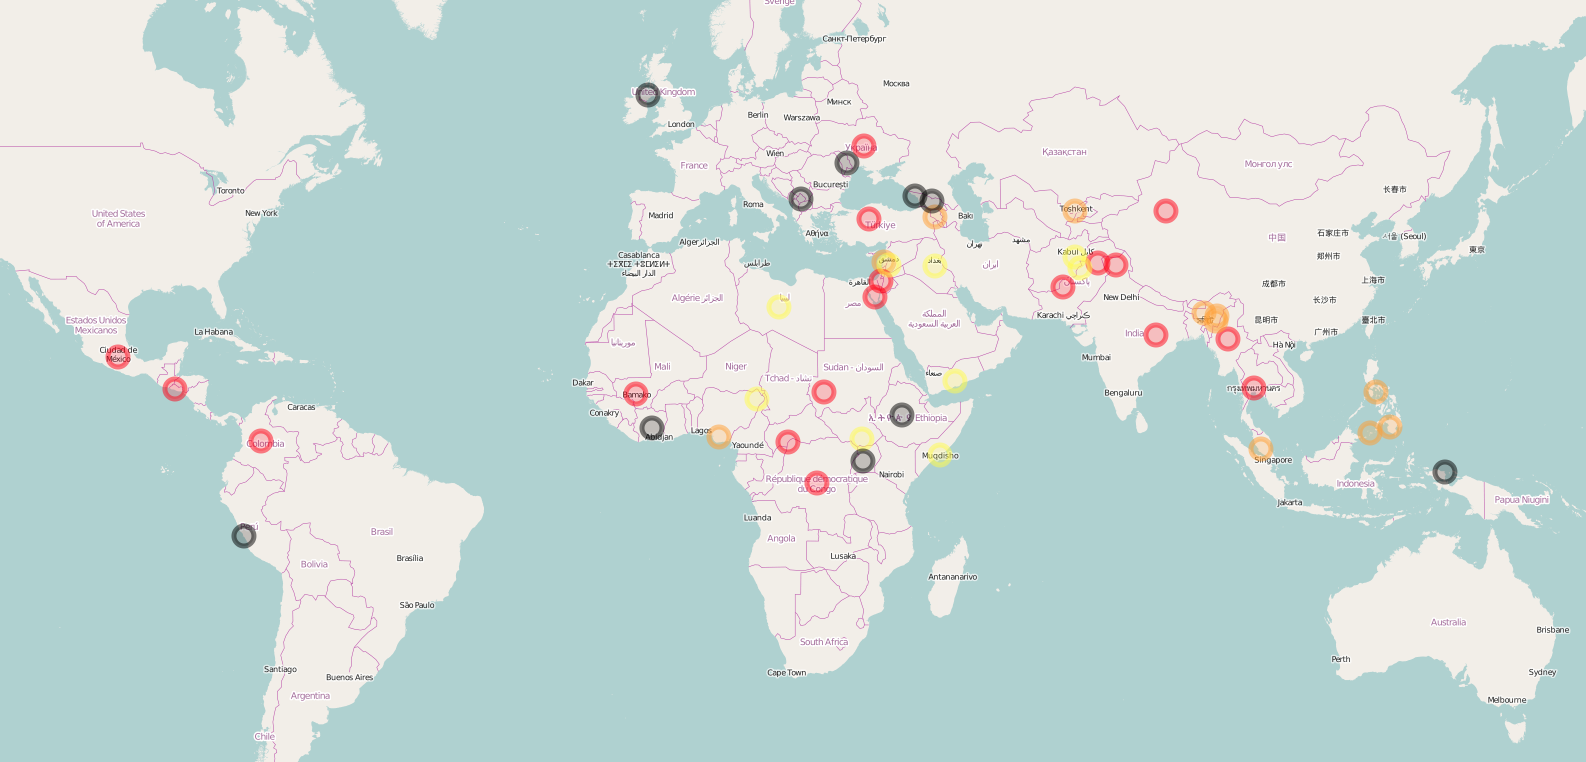
\includegraphics[width=0.9\columnwidth]{map.png}
\caption{A map of 48 conflicts. Black, yellow, orange and red circles indicate the level of intensity: archieved, low, medium and high, respectively.}
\label{rot}
\end{figure}

\subsection{Reddit Comment Dataset}
